\chapter{Implementacija i korisničko sučelje}
		
		
		\section{Korištene tehnologije i alati}
		
			\textbf{\textit{dio 2. revizije}}
			
			 \textit{Detaljno navesti sve tehnologije i alate koji su primijenjeni pri izradi dokumentacije i aplikacije. Ukratko ih opisati, te navesti njihovo značenje i mjesto primjene. Za svaki navedeni alat i tehnologiju je potrebno \textbf{navesti internet poveznicu} gdje se mogu preuzeti ili više saznati o njima}.
			
			
			\eject 
		
	
		\section{Ispitivanje programskog rješenja}
	
			
			\subsection{Ispitivanje komponenti}
			\textit{Ispitivanje komponenti ostvareno je korištenjem Jest alata za ispi-
                    tivanje. U nastavku su opisani provedeni testovi te priložene funkcija za tesriranje te izlaz koji se dobije testiranjem. Prikazani testovi pokrivaju klase UserModel i AppointmentModel koje implementiraju najvažnije funkcionalnosti aplikacije
                    }

            \begin{figure}[H]
                    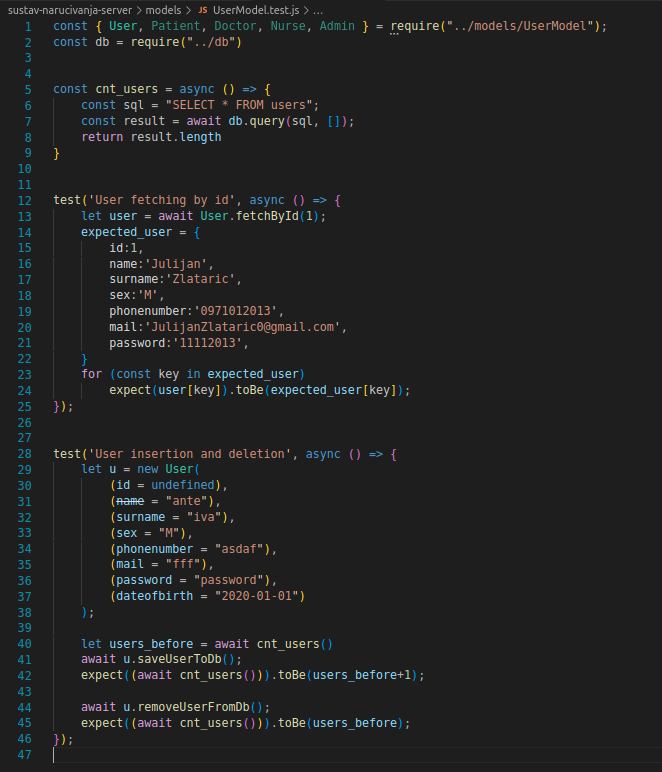
\includegraphics[width=300]{slike/usermodel_tests_code.png} %veličina u odnosu na širinu linije
                    \caption{Prikazani testovi testiraju dohvachanje usera iz baze podataka te njegovo ubacivanje i izbacivanje iz baze podataka. Navedene funkcionalnosti su nuzhne za pravilnu registraciju i login korisnika aplikacije.}
                    \label{fig:struktura} %label mora biti drugaciji za svaku sliku
                \end{figure}

                \begin{figure}[H]
                    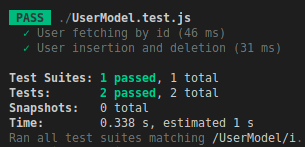
\includegraphics[width=\textwidth]{slike/usermodel_tests_out.png} %veličina u odnosu na širinu linije
                    \caption{Izlaz programa za testiranje klase UserModel s 2 testna primjera. Sa slike je vidljivo da klasa prolazi testne primjere.}
                    \label{fig:struktura} %label mora biti drugaciji za svaku sliku
                \end{figure}

            \begin{figure}[H]
                    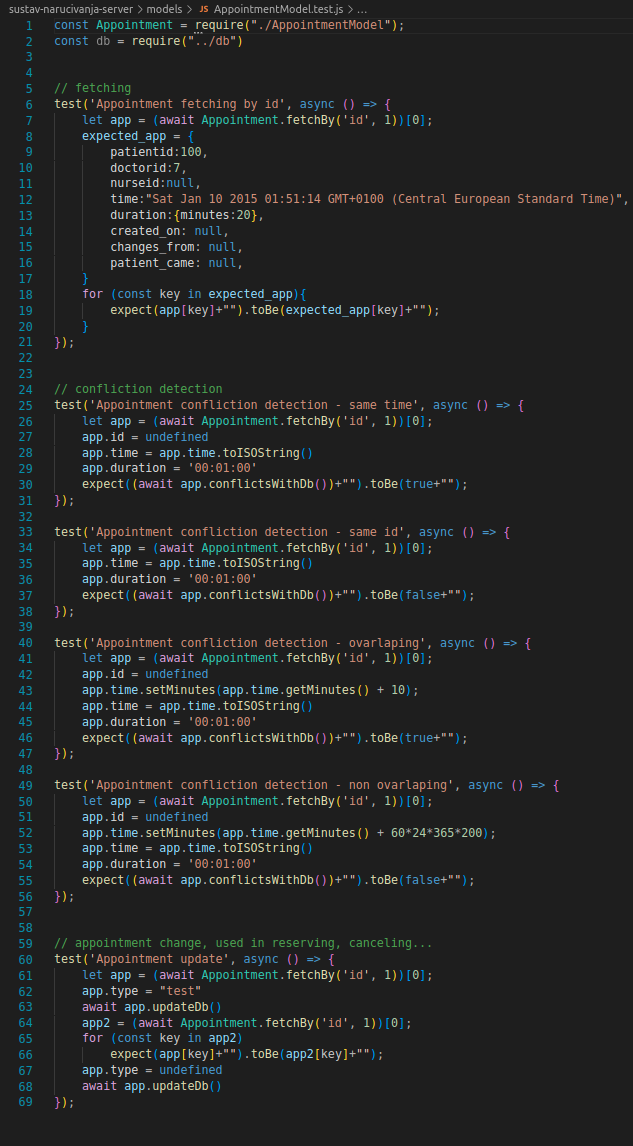
\includegraphics[width=300]{slike/appointment_tests_code.png} %veličina u odnosu na širinu linije
                    \caption{Prikazani testovi testiraju dohvachanje odredzenog termina iz baze podataka, testiranje postoji li odredzeni termin koji je u vremenskom konfliktu s odabranim terminom te testiranje updateanja termina. Testiranje konflikata ima vise rubnih sluchajeva, naime isti termin mogli smo vecz dohvatiti iz baze podataka te tada nebi trebalo biti konflikata, zatim mogucze je da se termin nalazi unutar drugoga, potpuno izvan...}
                    \label{fig:struktura} %label mora biti drugaciji za svaku sliku
                \end{figure}

                \begin{figure}[H]
                    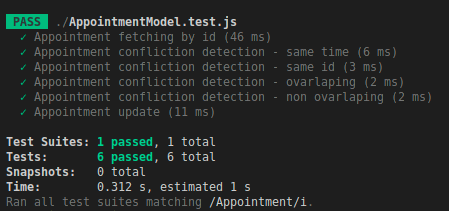
\includegraphics[width=\textwidth]{slike/appointment_tests_out.png} %veličina u odnosu na širinu linije
                    \caption{Izlaz programa za testiranje klase AppointmentModel s 6 testnih primjera. Sa slike je vidljivo da klasa prolazi testne primjere.}
                    \label{fig:struktura} %label mora biti drugaciji za svaku sliku
                \end{figure}
			
			
			
			\subsection{Ispitivanje sustava}
			
			 \textit{Potrebno je provesti i opisati ispitivanje sustava koristeći radni okvir Selenium\footnote{\url{https://www.seleniumhq.org/}}. Razraditi \textbf{minimalno 4 ispitna slučaja} u kojima će se ispitati redovni slučajevi, rubni uvjeti te poziv funkcionalnosti koja nije implementirana/izaziva pogrešku kako bi se vidjelo na koji način sustav reagira kada nešto nije u potpunosti ostvareno. Ispitni slučaj se treba sastojati od ulaza (npr. korisničko ime i lozinka), očekivanog izlaza ili rezultata, koraka ispitivanja i dobivenog izlaza ili rezultata.\\ }
			 
			 \textit{Izradu ispitnih slučajeva pomoću radnog okvira Selenium moguće je provesti pomoću jednog od sljedeća dva alata:}
			 \begin{itemize}
			 	\item \textit{dodatak za preglednik \textbf{Selenium IDE} - snimanje korisnikovih akcija radi automatskog ponavljanja ispita	}
			 	\item \textit{\textbf{Selenium WebDriver} - podrška za pisanje ispita u jezicima Java, C\#, PHP koristeći posebno programsko sučelje.}
			 \end{itemize}
		 	\textit{Detalji o korištenju alata Selenium bit će prikazani na posebnom predavanju tijekom semestra.}
			
			\eject 

           \begin{figure}[H]
                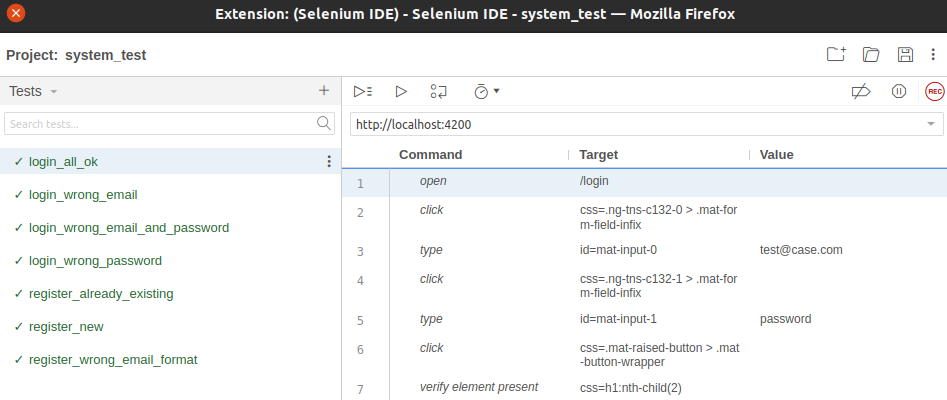
\includegraphics[width=\textwidth]{slike/tests_system/login_all_ok.png} %veličina u odnosu na širinu linije
                \caption{Program za testiranje.}
                \label{fig:struktura} %label mora biti drugaciji za svaku sliku
            \end{figure}

            \begin{figure}[H]
                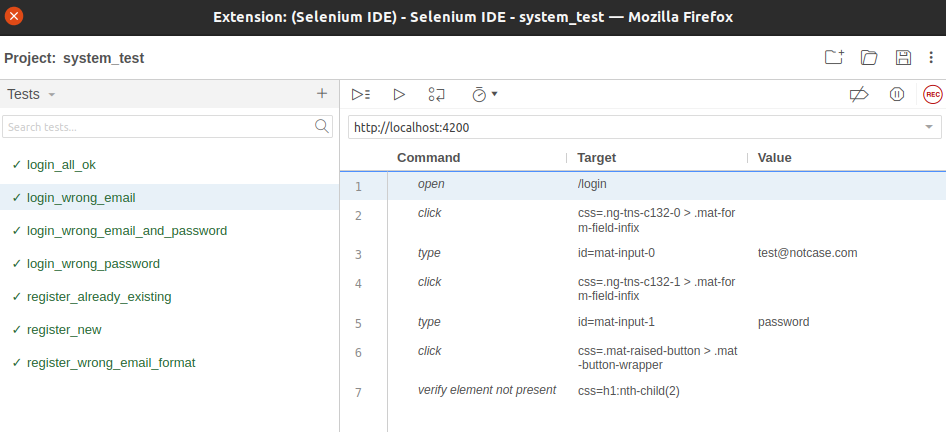
\includegraphics[width=\textwidth]{slike/tests_system/login_wrong_email.png} %veličina u odnosu na širinu linije
                \caption{Program za testiranje.}
                \label{fig:struktura} %label mora biti drugaciji za svaku sliku
            \end{figure}

            \begin{figure}[H]
                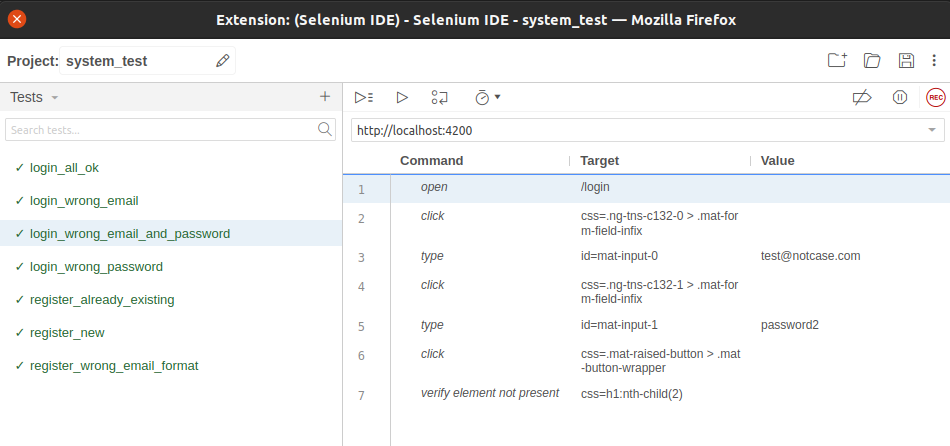
\includegraphics[width=\textwidth]{slike/tests_system/login_wrong_email_and_password.png} %veličina u odnosu na širinu linije
                \caption{Program za testiranje.}
                \label{fig:struktura} %label mora biti drugaciji za svaku sliku
            \end{figure}

            \begin{figure}[H]
                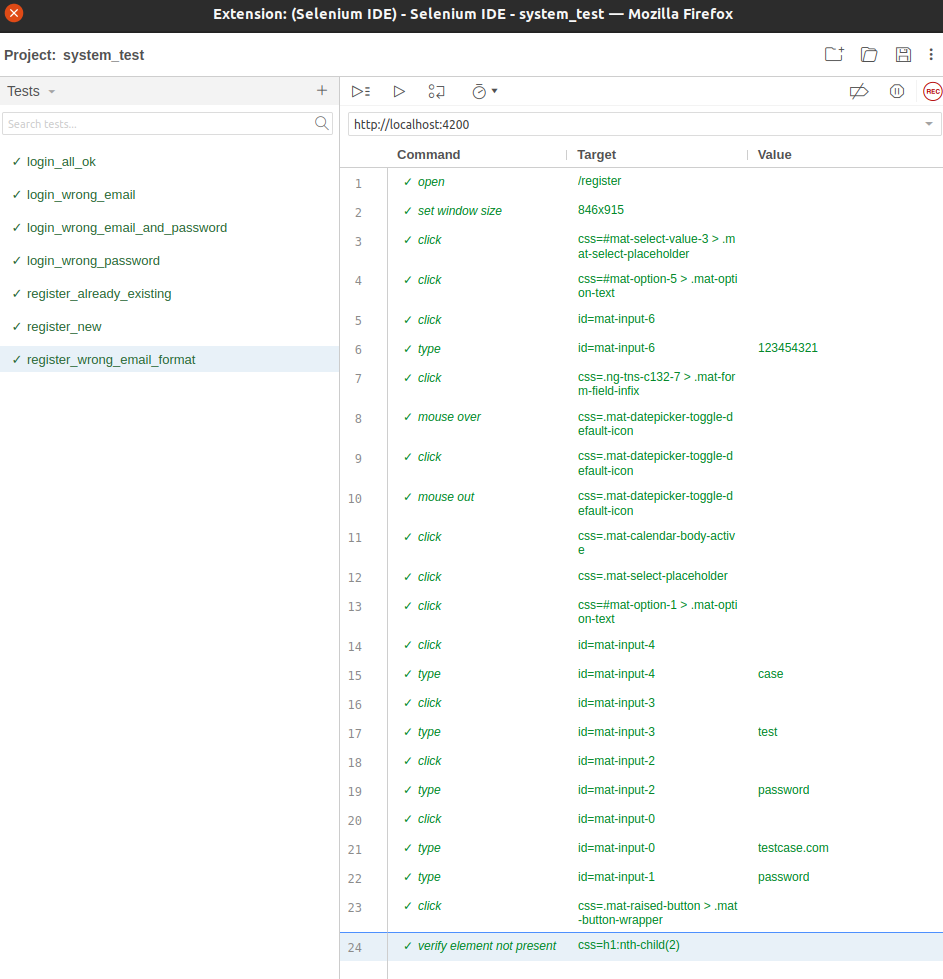
\includegraphics[width=\textwidth]{slike/tests_system/register_wrong_format.png} %veličina u odnosu na širinu linije
                \caption{Program za testiranje.}
                \label{fig:struktura} %label mora biti drugaciji za svaku sliku
            \end{figure}

            \begin{figure}[H]
                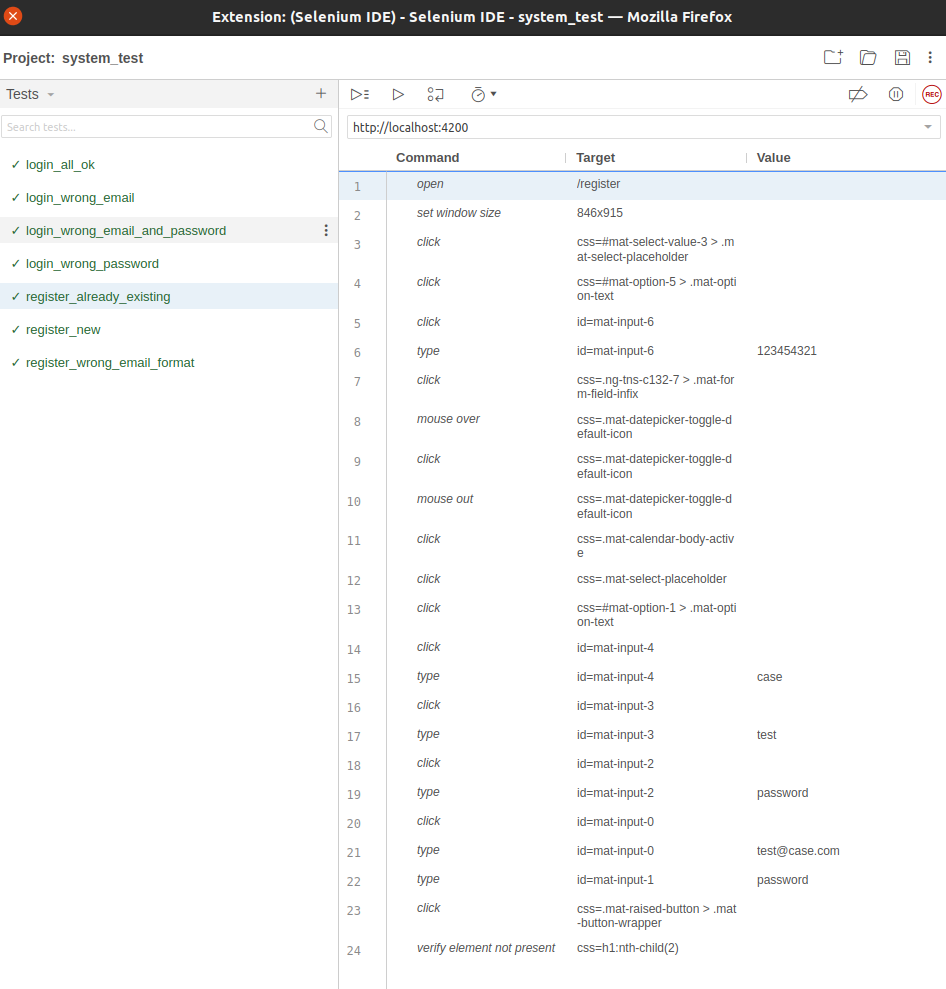
\includegraphics[width=\textwidth]{slike/tests_system/register_already_existing.png} %veličina u odnosu na širinu linije
                \caption{Program za testiranje.}
                \label{fig:struktura} %label mora biti drugaciji za svaku sliku
            \end{figure}

            \begin{figure}[H]
                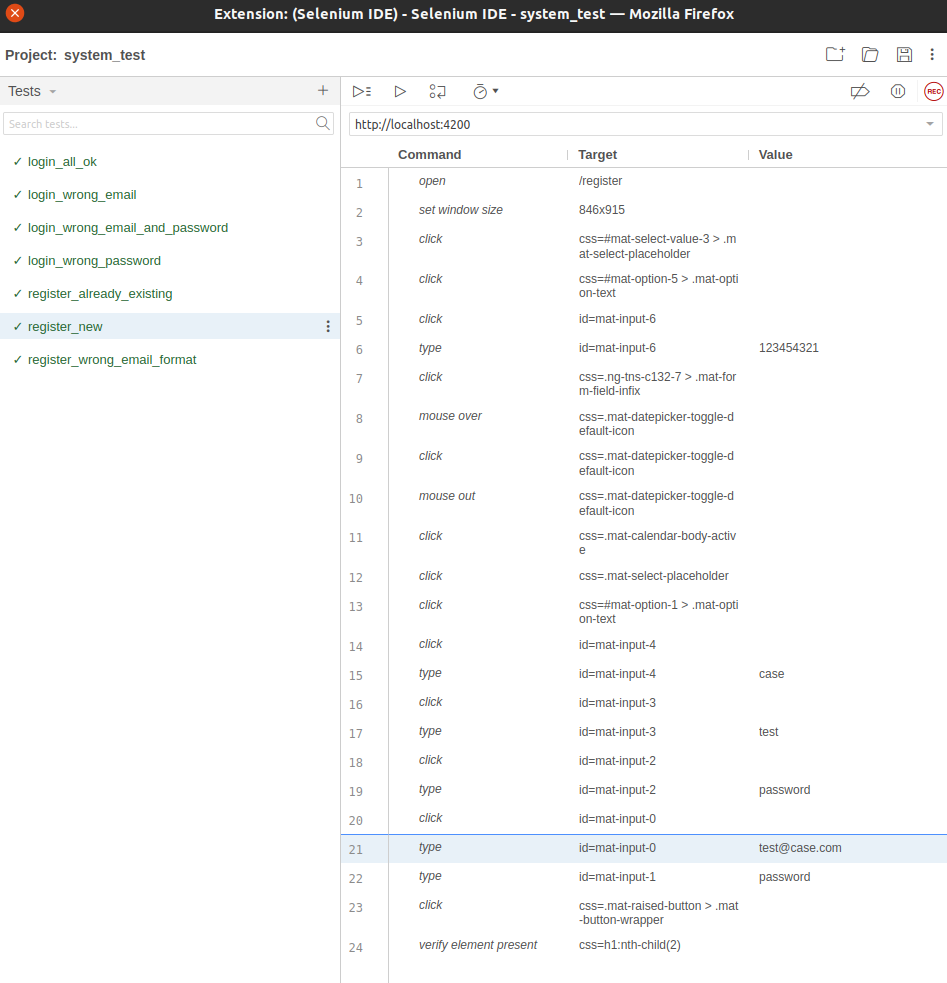
\includegraphics[width=\textwidth]{slike/tests_system/register_new.png} %veličina u odnosu na širinu linije
                \caption{Program za testiranje.}
                \label{fig:struktura} %label mora biti drugaciji za svaku sliku
            \end{figure}
		
		\section{Dijagram razmještaja}
			
			\textbf{\textit{dio 2. revizije}}
			
			 \textit{Potrebno je umetnuti \textbf{specifikacijski} dijagram razmještaja i opisati ga. Moguće je umjesto specifikacijskog dijagrama razmještaja umetnuti dijagram razmještaja instanci, pod uvjetom da taj dijagram bolje opisuje neki važniji dio sustava.}
			
			\eject 
		
		\section{Upute za puštanje u pogon}
		
			\textbf{\textit{dio 2. revizije}}\\
		
			 \textit{U ovom poglavlju potrebno je dati upute za puštanje u pogon (engl. deployment) ostvarene aplikacije. Na primjer, za web aplikacije, opisati postupak kojim se od izvornog kôda dolazi do potpuno postavljene baze podataka i poslužitelja koji odgovara na upite korisnika. Za mobilnu aplikaciju, postupak kojim se aplikacija izgradi, te postavi na neku od trgovina. Za stolnu (engl. desktop) aplikaciju, postupak kojim se aplikacija instalira na računalo. Ukoliko mobilne i stolne aplikacije komuniciraju s poslužiteljem i/ili bazom podataka, opisati i postupak njihovog postavljanja. Pri izradi uputa preporučuje se \textbf{naglasiti korake instalacije uporabom natuknica} te koristiti što je više moguće \textbf{slike ekrana} (engl. screenshots) kako bi upute bile jasne i jednostavne za slijediti.}
			
			
			 \textit{Dovršenu aplikaciju potrebno je pokrenuti na javno dostupnom poslužitelju. Studentima se preporuča korištenje neke od sljedećih besplatnih usluga: \href{https://aws.amazon.com/}{Amazon AWS}, \href{https://azure.microsoft.com/en-us/}{Microsoft Azure} ili \href{https://www.heroku.com/}{Heroku}. Mobilne aplikacije trebaju biti objavljene na F-Droid, Google Play ili Amazon App trgovini.}
			
			
			\eject 